\documentclass[11pt]{article} % scrbook otro formato
\usepackage[utf8]{inputenc}
\usepackage[spanish,es-tabla,es-nodecimaldot]{babel}

% Paquetes

\usepackage{amsmath}
\usepackage{amsthm}
\usepackage{amsfonts}
\usepackage{amssymb}
\usepackage{makeidx}
\usepackage{graphicx}
\usepackage{lmodern}
%\usepackage{kpfonts}
\usepackage{fancyhdr}
\usepackage{geometry}
\usepackage{lastpage}
\usepackage{subcaption}
\usepackage{array} % Para fjar tamaño de columnas
\RequirePackage{siunitx}
\usepackage{extramarks} % Para poder usar firstleftmarks
\usepackage[version=4]{mhchem} % Para poder usar formulas de reacciones nucleares
\usepackage{xcolor}
%\usepackage{newtxtext, newtxmath} % Cambia la fuente (pero mola)

%##############################################################################
%######### Ponemos el decimal con . ###########################################
%##############################################################################

\sisetup{output-decimal-marker={.},
	% exponentes ------------------------
	%exponent-mode=threshold,
	%exponent-thresholds=-3:2, % non usar exponentes 10^{-2,-1, 0, 1}
	% redondear -------------------------
	% round-mode=figures, % cifras sig
	% round-mode=places, % cantos decimales
	round-mode=uncertainty, % cifras sig da incerteza (necesario usar erro)
	round-precision=2,
	uncertainty-mode = separate,
	print-unity-mantissa=false,
	% unidades --------------------------
	inter-unit-product = \ensuremath{{}\cdot{}}, % separacion entre unidades
	% per-mode=power-positive-first, % so furrula con metodo interpretado puro
	inline-per-mode=single-symbol,
	display-per-mode=fraction,
}

%##############################################################################
%######### Para codigo python #################################################
%##############################################################################

\definecolor{codegreen}{rgb}{0,0.6,0}
\definecolor{codegray}{rgb}{0.5,0.5,0.5}
\definecolor{codepurple}{rgb}{0.58,0,0.82}
\definecolor{backcolour}{rgb}{0.95,0.95,0.92}

\usepackage{listings}


\lstdefinestyle{mystyle}{	backgroundcolor=\color{backcolour},   	commentstyle=\color{codegreen},	keywordstyle=\color{magenta},	numberstyle=\tiny\color{codegray},	stringstyle=\color{codepurple},	basicstyle=\ttfamily\footnotesize,	breakatwhitespace=false,         	breaklines=true,                 	captionpos=b,                    	keepspaces=true,                 	numbers=left,                    	numbersep=5pt,                  	showspaces=false,                	showstringspaces=false,	showtabs=false,                  	tabsize=2}

\lstset{style=mystyle}
%\usepackage{background}     % Para manejar el fondo


%##############################################################################
%######### Tipo de fuente #################################################
%##############################################################################

%\usepackage{kpfonts}

%\usepackage{helvet} 
%\renewcommand{\familydefault}{\sfdefault}.

%\usepackage{fontspec} % Paquete necesario para seleccionar fuentes
%\setmainfont{Verdana} % Cambia la fuente principal a Verdana


%##############################################################################
%######### Geometría #################################################
%##############################################################################

\geometry{a4paper, total={152mm,237mm}, left=31mm, top=30mm}



%##############################################################################
%######### Formatos capítulo #################################################
%##############################################################################

%\usepackage[lmodern]{quotchap}
%\usepackage[Bjornstrup]{fncychap}

% Para el Bjornstrup
%\ChNumVar{\fontsize{76}{80}\usefont{OT1}{pzc}{m}{n}\selectfont}
%\ChTitleVar{\raggedright\Huge\sffamily\bfseries}


%##############################################################################
%######### Hiperreferenias #################################################
%##############################################################################


\usepackage[colorlinks=true,allcolors=blue]{hyperref} % Crea las


%##############################################################################
%######### Formato de pagina #################################################
%##############################################################################

%\renewcommand{\chaptermark}[1]{\markboth{\chaptername\ \thechapter.\ #1}{}}
\renewcommand{\sectionmark}[1]{\markright{\thesection.\ #1}}

\setlength{\headsep}{27pt} % Distancia entre la cabezera y el texto
\setlength{\footskip}{30pt} % Distancia entre el pie de pagina y el texto
\pagestyle{fancy}
\fancyhf{}
\fancyhead[LE]{\rightmark} % L,R,C-> left, right, center [LE,RO]
\fancyhead[RO]{\rightmark} % E,O -> even (par), odd (impar)
\fancyhead[LO,RE]{Daniel Vázquez Lago}
\fancyfoot[CE,CO]{\thepage}
\renewcommand{\headrulewidth}{1pt} % Cambiamos el grosor de la linea de arriba
\renewcommand{\footrulewidth}{0pt}



%##############################################################################
%#########  Modificar caption #################################################
%##############################################################################

\usepackage[font=small, justification=centering]{caption}  % Configura las captions



%##############################################################################
%######### Comandos propios #################################################
%##############################################################################

\newcommand{\parentesis}[1]{\left( #1  \right)} 
\newcommand{\parciales}[2]{\frac{\partial #1}{\partial #2}}
\newcommand{\pparciales}[2]{\parentesis{\parciales{#1}{#2}}}
\newcommand{\ccorchetes}[1]{\left[ #1  \right]}
\newcommand{\D}{\mathrm{d}}
\newcommand{\derivadas}[2]{\frac{\D #1}{\D #2}}

\newcommand{\tquad}{\quad \quad \quad}
\newcommand{\vnabla}{\vec{\nabla}}

\newcommand{\Ocal}{\mathcal{O}}
\newcommand{\Ncal}{\mathcal{N}}
\newcommand{\Hcal}{\mathcal{H}}

\newcommand{\logd}{\log_{10}}

\newcommand{\eV}{\text{eV}}
\newcommand{\cm}{\text{cm}}
\newcommand{\cmm}{\text{cm}^{-1}}
\newcommand{\fm}{\text{fm}}
\newcommand{\He}{\text{He}}
\newcommand{\p}{\text{p}}
\newcommand{\e}{\text{e}}
\newcommand{\cte}{\text{cte}}


% Comandos vectoriales

\newcommand{\an}{\mathbf{a}}
\newcommand{\bn}{\mathbf{b}}
\newcommand{\dn}{\mathbf{d}}
\newcommand{\jn}{\mathbf{j}}
\newcommand{\lnn}{\boldsymbol{\ell}}
\newcommand{\lnnn}{\boldsymbol{l}}
\newcommand{\kn}{\mathbf{k}}
\newcommand{\pn}{\mathbf{p}}
\newcommand{\qn}{\mathbf{q}}
\newcommand{\rn}{\mathbf{r}}
\newcommand{\sn}{\mathbf{s}}
\newcommand{\un}{\mathbf{u}}
\newcommand{\vn}{\mathbf{v}}
\newcommand{\xn}{\mathbf{x}}
\newcommand{\yn}{\mathbf{y}}
\newcommand{\qndot}{\dot{\qn}}

\newcommand{\unovec}{\vec{\mathbf{1}}}

\newcommand{\alphan}{\boldsymbol{\alpha}}
\newcommand{\sigman}{\boldsymbol{\sigma}}
\newcommand{\pin}{\boldsymbol{\pi}}


\newcommand{\An}{\mathbf{A}}
\newcommand{\Bn}{\mathbf{B}}
\newcommand{\En}{\mathbf{E}}
\newcommand{\Gn}{\mathbf{G}}
\newcommand{\Jn}{\mathbf{J}}
\newcommand{\Kn}{\mathbf{K}}
\newcommand{\Ln}{\mathbf{L}}
\newcommand{\Rn}{\mathbf{R}}
\newcommand{\Sn}{\mathbf{S}}
\newcommand{\Tn}{\mathbf{T}}
\newcommand{\In}{\mathbf{I}}

\newcommand{\hnn}{\hat{\mathbf{n}}}
\newcommand{\hnr}{\hat{\mathbf{r}}}
\newcommand{\hnz}{\hat{\mathbf{z}}}
\newcommand{\hnx}{\hat{\mathbf{x}}}
\newcommand{\hny}{\hat{\mathbf{y}}}
\newcommand{\hnu}{\hat{\mathbf{u}}}
\newcommand{\hnR}{\hat{\mathbf{R}}}
\newcommand{\hnv}{\hat{\mathbf{v}}}
\newcommand{\hnk}{\hat{\mathbf{k}}}
\newcommand{\hni}{\hat{\mathbf{i}}}
\newcommand{\hnj}{\hat{\mathbf{j}}}
\renewcommand{\hnk}{\hat{\mathbf{k}}}





%##############################################################################
%######### Teoremas/definiciones #################################################
%##############################################################################

%\theoremstyle{definition}
%\newtheorem{definition}{Definición}[chapter]
%\theoremstyle{theorem}
%\newtheorem{theorem}{Teorema}[chapter]




%##############################################################################
%######### Referncia para euccaiones y figuras ################################
%##############################################################################

%\numberwithin{equation}{section}
%\numberwithin{figure}{section}




%##############################################################################
%######### Documento #################################################
%##############################################################################


\author{Daniel Vazquez Lago}
\title{Simulación en física de materiales}


\begin{document}	
	
\maketitle
\newpage
\tableofcontents
\section{Objetivos}
	
El objetivo de este primer optativo es estudiar si realmente, tras los $\num{5e5}$ pasos, hemos llegado a una configuración de equilibrio. Para esto presentaremos 3 diferentes condiciones que un sistema aislado en equilibrio debería satisfacer (\cite{Haile}):

\begin{itemize}
 	\item La energía $E$ total debe mantenerse constante en el tiempo, a poder ser $E=-575$.
 	\item Los valores medios de las velocidades (cada una de las componentes) deben seguir distribuciones de Maxwell.
 	\item La función $H$ de Boltzmann debe tender a un valor constante. 	
\end{itemize}
Existen mas condiciones que no trataremos aquí, no por otra cosa que la falta de información. Sin embargo, ninguna de estas (individualmente y colectivamente) nos garanticen de manera completamente inequívoca que estamos en el equilibrio.
	
\section{Equilibración}

En esta sección vamos a estudiar desde una perspectiva teórica cuales son las condiciones de equilibrio, para luego ver cuales son los resultados (y la implementación) según cada una de estas condiciones. En esta sección usaremos sobretodo el contenido que aparece en las páginas 206-209 del Haile \cite{Haile}. 

\subsection{Energía total constante}

\subsubsection{Teoría}

Esta condición nos asegura que el si $E$ es constante en el tiempo, de tal manera que las fluctuaciones de la energía cinética y energía potencial deben ser contrarias, esto es, cuando una de ellas aumente la otra debe disminuir y viceversa. 

\subsubsection{Resultados e implementación}

Esta es, de las tres condiciones, la que mas sencilla es de implementar, ya que en el obligatorio 2 ya se nos exigía escribir los distintos valores de la energía para cada una de las interacciones (incluida la que venía de la fcc). En este caso lo único que debemos hacer es leer los datos almacenados en el \texttt{.dat} para luego hacer las gráficas (usando matplotlib.pyplot), y obtener el valor medio de las energías, también en python. Los valores medios de las energías totales y cinéticas (las cinéticas serán interesantes para la siguiente condición de equilibrio):

\begin{table}[h!] \centering
	\begin{tabular}{c|c|c|c|c}
		& $E_t$ & $s(E_t)$ & $E_{cin}$ & $s(E_ {cin})$ \\ \hline
		$1^o$ &-575.0422 & 6.9e-09 & 1094.15 & 2.5e-08 \\ \hline
		$2^o$ & -575.0044 & 1.0e-08 & 1091.00 & 1.8e-08 
	\end{tabular}
	\caption{Valores de las medias para cada interacción e incertidumbre asociada a la media.}
	\label{Tab:01}
\end{table}
Una vez tenemos estos datos podemos entender mejor porque realizamos una segunda interacción. Dado que nosotros queremos una dinámica molecular que oscile sobre -575, queremos que el valor medio de $E_{t}$ se parezca lo más posible a -575. Por ello que oscilase en la 2a cifra decimal no nos parecía suficiente. \\

Aún con todo, podemos ver que las oscilaciones respecto la media son muy pequeñas, por lo que en ambas configuraciones se verifica la condición de estabilidad en la energía del equilibrio, aunque no el mismo equilibrio (ambas pertenecen a colectividades microcanónicas diferentes, ya que la NVE depende de E y en E es diferente en las dos equilibraciones).


\begin{figure}[h!] \centering
\begin{subfigure}{0.45\linewidth} \centering
	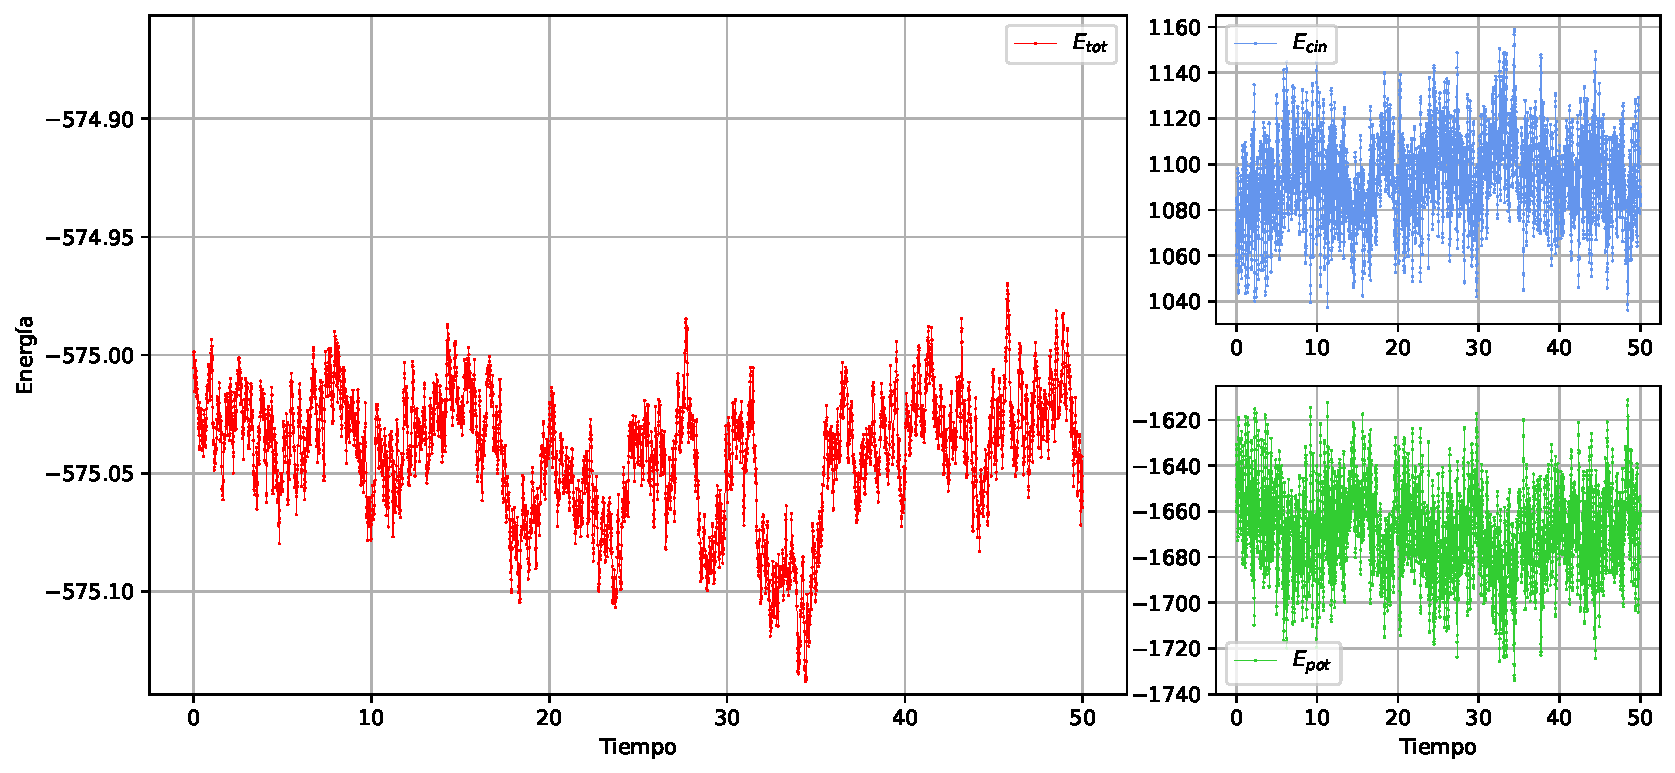
\includegraphics[width=1\textwidth]{../../Graficas/Et-equilibra-500K-1.pdf}
	\caption{Primeros 500K pasos.}
	\label{Fig:01}
\end{subfigure}	
\begin{subfigure}{0.45\linewidth}\centering
	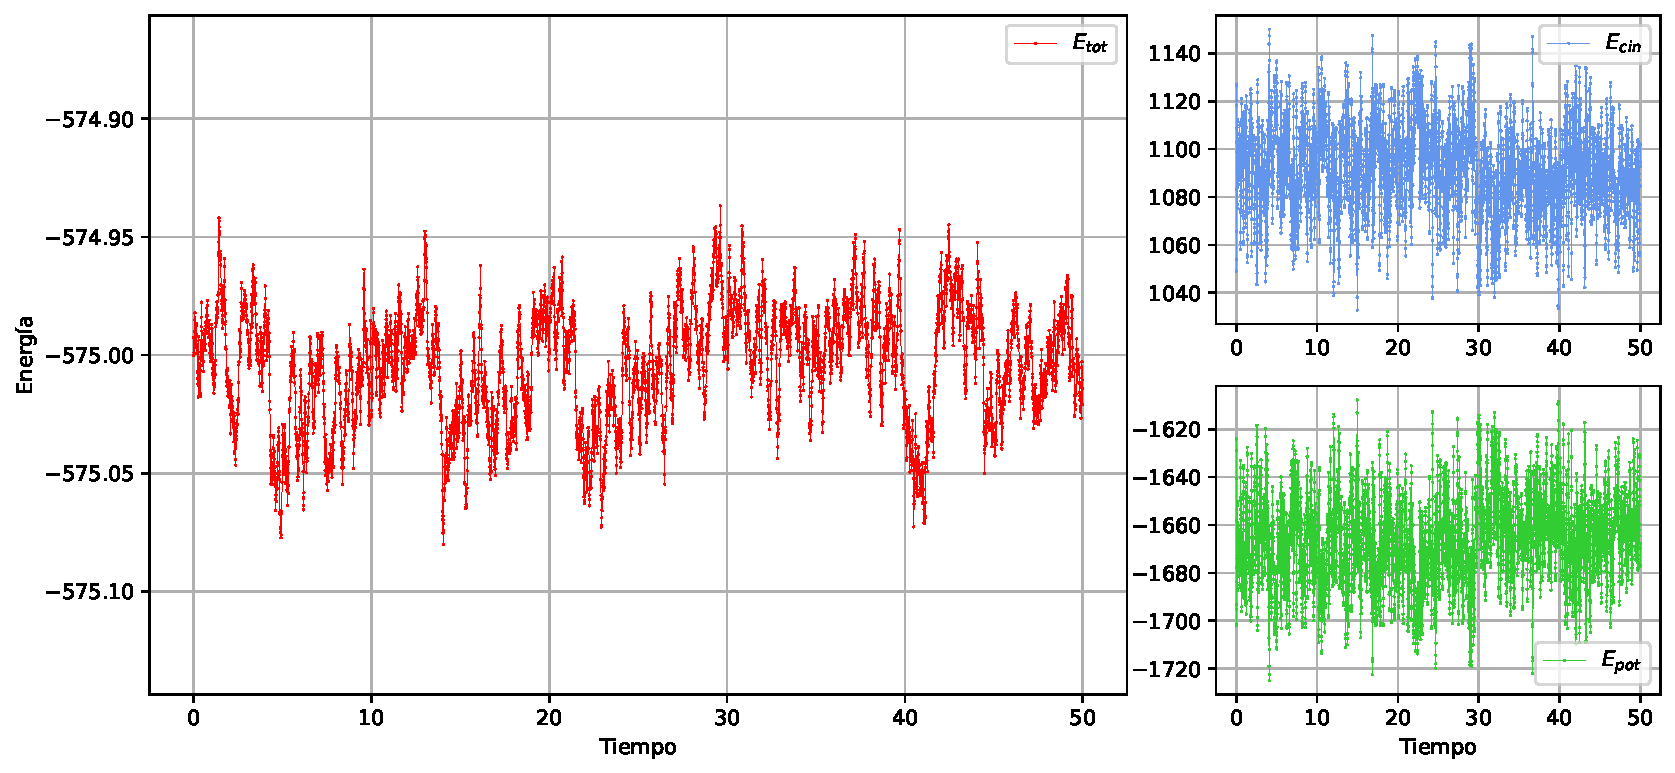
\includegraphics[width=1\textwidth]{../../Graficas/Et-equilibra-500K-2.pdf}
	\caption{Segundos 500K pasos.}
	\label{Fig:02}
	\end{subfigure}	
\caption{Evolucion de la energía total (y cinética y potencial) para los primeros 500K pasos y para los segundos 500K pasos.}
\end{figure}


	
\subsection{Distribución de Velocidades}
	
\subsubsection{Teoría}

En este apartado vamos a seguir el desarrollo hecho en el \cite{Haile} (pag. 65-66, pag. 120). Para una distribución de velocidades en el equilibrio (colectividad NVT) verifica que, para cada una de las componentes $i$ de las velocidades ($v_x,v_y,v_z$), dado que son independientes: 

\begin{equation}
	f(v_i) = \sqrt{\frac{m}{2\pi k T}} \exp \parentesis{- \frac{mv_i^2}{2kT}}
\end{equation}
Aunque la distribución de Maxwell halla sido derivada en el formalismo de la colectividad canónica (NVT, PVT...), la distribuciones de cualquier sistema en el equilibrio debería ser de este tipo, ya que en el límite termodinámico las propiedades en las diferentes colectividades se vuelven equivalentes. \\

Una de las consecuencias de la distribución de velocidades es la equipartición de la energía, por lo las componentes cartesianas de la velocidades moleculares deberían tener un valor medio igual al de la temperatura del sistema:

\begin{eqnarray}
	\frac{1}{N} \left\langle \sum_i v_{ix}^2 \right\rangle = 
	\frac{1}{N} \left\langle \sum_i v_{ix}^2 \right\rangle = 
	\frac{1}{N} \left\langle \sum_i v_{ix}^2 \right\rangle = T
\end{eqnarray}

\subsubsection{Implementación}

Para implementar correctamente el programa necesitamos primero saber que tenemos y que queremos obtener. Como bien dijimos en el anterior apartado, queremos obtener una distribución de velocidades, para verificar si tiene un comportamiento gaussiano o cuasi-gaussiano (y ver si coinciden las distribuciones para los diferentes ejes, ya que en el caso de que no coincidan sabremos que la simulación no es correcta). Tenemos en total 2.5M de velocidades por eje, ya que hemos guardado 5001 interacciones (desde $t=0$ hasta $t=50$ teniendo en cuenta que $\Delta t= 10^{-4}$ y que almacenamos los datos de las velocidades cada 100 interacciones). \\

Entonces lo que debemos hacer en el programa es lo siguiente:

\begin{enumerate}
	\item Leemos los diferentes valores de las velocidades, y las apilamos todas en un mismo array (no vamos a estudiar la evolución temporal de la distribución, si no la distribución global). 
	\item Definimos los parámetros del histograma:
	\begin{itemize}
		\item Número de intervalos/bins. Nosotros usaremos la fórmula clásica: el número de intervalos será la raíz cuadrada del número total de valores. En nuestro caso entonces tendremos $1582$ intervalos. 
		\item Límites de la muestra. Para calcular los límites de la muestra cogimos el valor mas grande (en absoluto) de todas las velocidades posibles (7.5M datos), y lo usamos tanto como valor máximo y valor mínimo de la muestra.
		\item Ancho de los bins. Calculamos la anchura total de la muestra (límite superior menos límite inferior) y lo dividimos por el número de bins total.
		\item Valor medio de cada bin. Valor al que asociaremos las velocidades más proximas. De define como el valor mitad entre el límite superior e inferior de un bin. 
		\item Frecuencias. Cada bin tendrá asociada una frecuencia en función de la cantidad de valores que haya más próximos al valor medio del mismo que a cualquier otro.
	\end{itemize}
	\item Una vez definidos los valores procedemos a rellenar los histogramas (esto es, definir la frecuencia de cada bin). Nosotros lo que hicimos fue hacer un bucle para cada velocidad (3 bucles), donde leemos paso por paso cada una de los valores de las velocidades (por esa misma razón las tuvimos que apilar), de tal manera que en cada interacción recorra cada uno de los bins, viendo si es más pequeño que el límite superior del bin, empezando por el más pequeño. En el momento que encontramos el bin al que asociar dicho valor, salimos del bucle. La implemetnación en fortran es pequeña:
\begin{lstlisting}[language=Fortran]
do i=1,500*5001
  v=vxx(i)   
  do j=1,kintervalos_int
	if (v<=-distancia/2.d00+intervalo*j) then
	  histx(j)=histx(j)+1.d00
	  exit
	endif   
  enddo     
enddo
\end{lstlisting}
	\item Una vez tenemos la frecuencia, guardamos en 3 archivos el valor medio de cada bin y la frecuencia asociada, de tal modo que tenemos ya nuestros histogramas. Cada archivo contiene el histograma de cada una de las velocidades.
	
\end{enumerate}
Cabe destacar que nosotros no usamos el algoritmo mas eficiente posible para obtener la frecuencia de los bins, pero si el más sencillo de implementar. De tener mas datos habría que cambiar el método. En general no es un programa eficiente, pero funciona, y dado que el tiempo de cálculo es pequeño\footnote{Entre 5-6 segundos.}, no es relevante.


\subsubsection{Resultados}

Las gráficas obtenidas a partir de los resultados dados por  fortran se hicieron en python mediante un programa que leía directamente del \texttt{.dat}. Como hemos mencionado, hicimos dos interacciones. En ambas, tal y como se puede ver en las gráficas, para ambas las distribuciones coinciden entre sí, lo cual es un buen indicio. 

\begin{figure}[h!] \centering
\begin{subfigure}{0.45\linewidth} \centering
	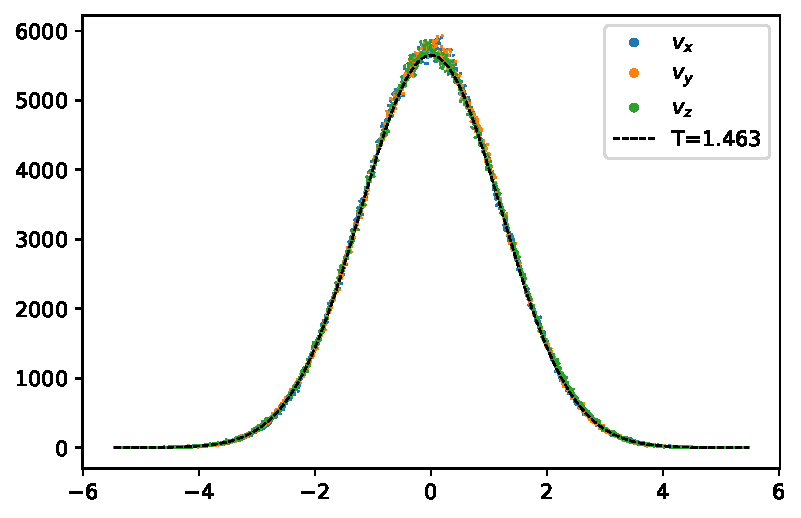
\includegraphics[width=1\textwidth]{../../Graficas/Velocidades_histo_1.pdf}
	\caption{primeros 500K pasos.}
	\label{Fig:03}
\end{subfigure}	
\begin{subfigure}{0.45\linewidth} \centering
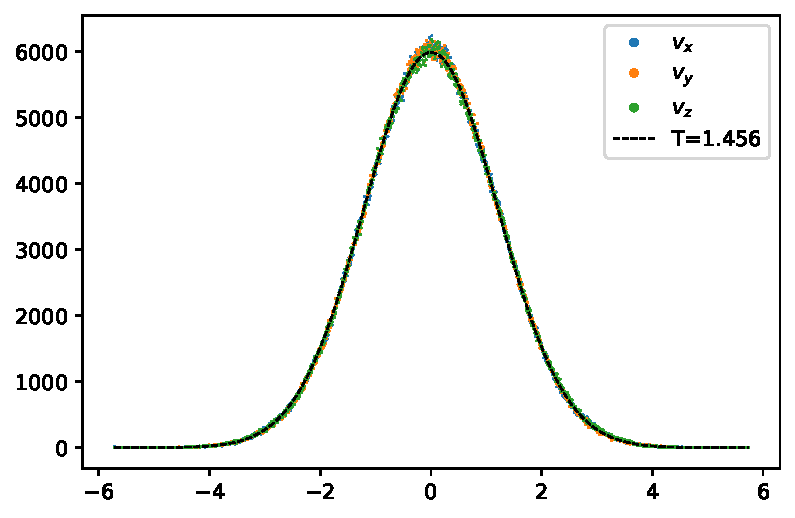
\includegraphics[width=1\textwidth]{../../Graficas/Velocidades_histo_2.pdf}
\caption{segundos 500K pasos.}
\label{Fig:04}
\end{subfigure}	
\caption{valores de la distribución de velocidades para cada eje, con la distribución de Maxwell asociada. Como podemos ver el resultado no está normalizado.}
\end{figure}

Veamos ahora si coinciden con la distribución de Maxwell asociada. Para calcular la temperatura necesaria para saber la distribución de Maxwell de las velocidades usamos la energía cinética media anteriormente calculada. Como podemos ver la distribución de Maxwell encaja casi de manera perfecta en ambas distribuciones, lo cual significa que verifican la condición previamente dicha.

\begin{equation}
	T = \frac{2\langle E_{cin} \rangle}{fk}
\end{equation}
donde $f$ es el número de grados de libertad del sistema y $k$ la constante de Boltzmann. Supondremos que es un valor suficientemente bueno.

	
\subsection{Distribución $H$-Boltzmann} 	
\subsubsection{Teoría}

En este apartado vamos a seguir el desarrollo hecho en el \cite{Haile} (pag. 66-67, pag. 120-121). Definimos la función $H$ de Boltzmann (función $H$) en un instante $t$ como:

\begin{eqnarray}
	H_i(t) = \int_{-\infty}^{\infty} f(v_i) \ln (f(v_i)) \D v_i \tquad i = x,y,z
\end{eqnarray} 
de tal modo que podemos definir la $H$ de Boltzmann como
\begin{eqnarray}
	H=\frac{1}{3} \parentesis{H_x+H_y+H_z}
\end{eqnarray}

El \textbf{teorema H de Boltzmann} asegura que una distribución llega al equilibrio cuando se alcanza un mínimo en la función $H$ de Boltzmann, dada por la anterior ecuación. Sin embargo nosotros no podemos implementar integrales, si no sumatorios (las integrales tienen un carácter infinitesimal que no podemos alcanzar con el ordenador), por lo que nosotros tendremos que implementar:

\begin{equation}
	H_i (t) = \sum_{\Delta v_i} f(v_i) \ln (f(v_i)) \Delta v_i  \tquad i=x,y,z
\end{equation}
donde

\begin{equation}
	f(v_x) \Delta v_x = \frac{1}{N} \sum_i^N \delta (v_x-v_{xi}) \Delta v_x
\end{equation}
e igual para $v_y$ e $v_z$. 

\subsubsection{Implentación}

La implementación es prácticamente idéntica a la de la distribución de velocidades, salvo por el último paso. Para implementar correctamente el programa necesitamos primero saber que tenemos y que queremos obtener. Como bien dijimos en la teoría, queremos obtener la función $H$ de Boltzmann, ya que $H$ se mantenga constante en el tiempo es una condición para que estemos en el equilibrio. La función $H$ de bolztmann se obtiene conociendo la distribución de de velocidades en un instante temporal determinado, por lo que lo que deberemos cambiar es el final del programa

Entonces lo que debemos hacer en el programa es lo siguiente:

\begin{enumerate}
	\item Leemos los diferentes valores de las velocidades, y las apilamos todas en un mismo array (no vamos a estudiar la evolución temporal de la distribución, si no la distribución global). 
	\item Definimos los parámetros del histograma:
	\begin{itemize}
		\item Número de intervalos/bins. En este caso bamos a disminuir el número de bins. En este caso cogeremos entorno a 200 bins, de tal modo que $\Delta x\approx 0.05$. Hacemos esto por que el Haile \cite{Haile} usa este, y queremos comparar los datos obtenidos (pag. 121) con sus resultados, aunque el use un modelo de esferas duras en esa páginas.
		\item Límites de la muestra. Igual que en distribución de velocidades.
		\item Ancho de los bins. Igual que en distribución de velocidades.
		\item Frecuencias. Igual que en distribución de velocidades.
	\end{itemize}
	\item Una vez definidos los valores procedemos a rellenar los histogramas (esto es, definir la frecuencia de cada bin). Nosotros lo que hicimos fue hacer un bucle para cada velocidad (3 bucles), donde leemos paso por paso cada una de los valores de las velocidades (por esa misma razón las tuvimos que apilar), de tal manera que en cada interacción recorra cada uno de los bins, viendo si es más pequeño que el límite superior del bin, empezando por el más pequeño. Dado que tenemos que implementar la evolución temporal, lo que haremos, a diferencia del anterior, es incluir un if al final del segundo lazo, de tal manera que si llevamos ya 500 partículas ponga a cero el histograma, y guarde el valor de $H_i(t)$. Podemos ver de manera sencilla la implementación:

\begin{lstlisting}[language=Fortran]
do i=1,500*5001
  v=vxx(i)   
  do j=1,kintervalos_int
    if (v<=-distancia/2.d00+intervalo*j) then
      histx(j)=histx(j)+1.d00
      exit
    endif   
  enddo     
  if (modulo(i,500).eq.0) then 
    do j=1,kintervalos_int
      if (histx(j).ne.0.d00) then
        Hx(int(i/500))=Hx(int(i/500))+intervalo*(log(histx(j)/np))*histx(j)/np
      endif    
    enddo     
    histx=0.d00
  endif  
enddo
\end{lstlisting}
	\item Una vez tenemos $H_x(t),H_y(t),H_z(t)$ los escribimos en el \texttt{.dat}.
	
\end{enumerate}
Cabe destacar que nosotros no usamos el algoritmo mas eficiente posible para obtener la frecuencia de los bins, pero si el más sencillo de implementar. De tener mas datos habría que cambiar el método. En general no es un programa eficiente, pero funciona, y dado que el tiempo de cálculo es pequeño\footnote{Entre 5-6 segundos.}, no es relevante. 

\subsubsection{Resultados}

Los valores de la dispersión $\Delta$ de $H(t)$ los valores vienen dados por

\begin{equation}
	\Delta_1 =  0.000583 \tquad \Delta_2 = 0.000599
\end{equation}
como podemos ver son muy pequeños, casi podemos asumir $H(t)$ constante. En las gráficas también se puede ver como estos valores oscilan respecto a un mismo valor, incluso para los primeros 500K pasos desde el principio, lo cual es muy sorprendente, ya que no debería estar tan próximo al equilibrio al principio. En cualquier caso, es evidente que se mantiene con el tiempo en ambas configuraciones, por lo que ambas cumplen esta condición. 

	
\begin{figure}[h!] \centering
	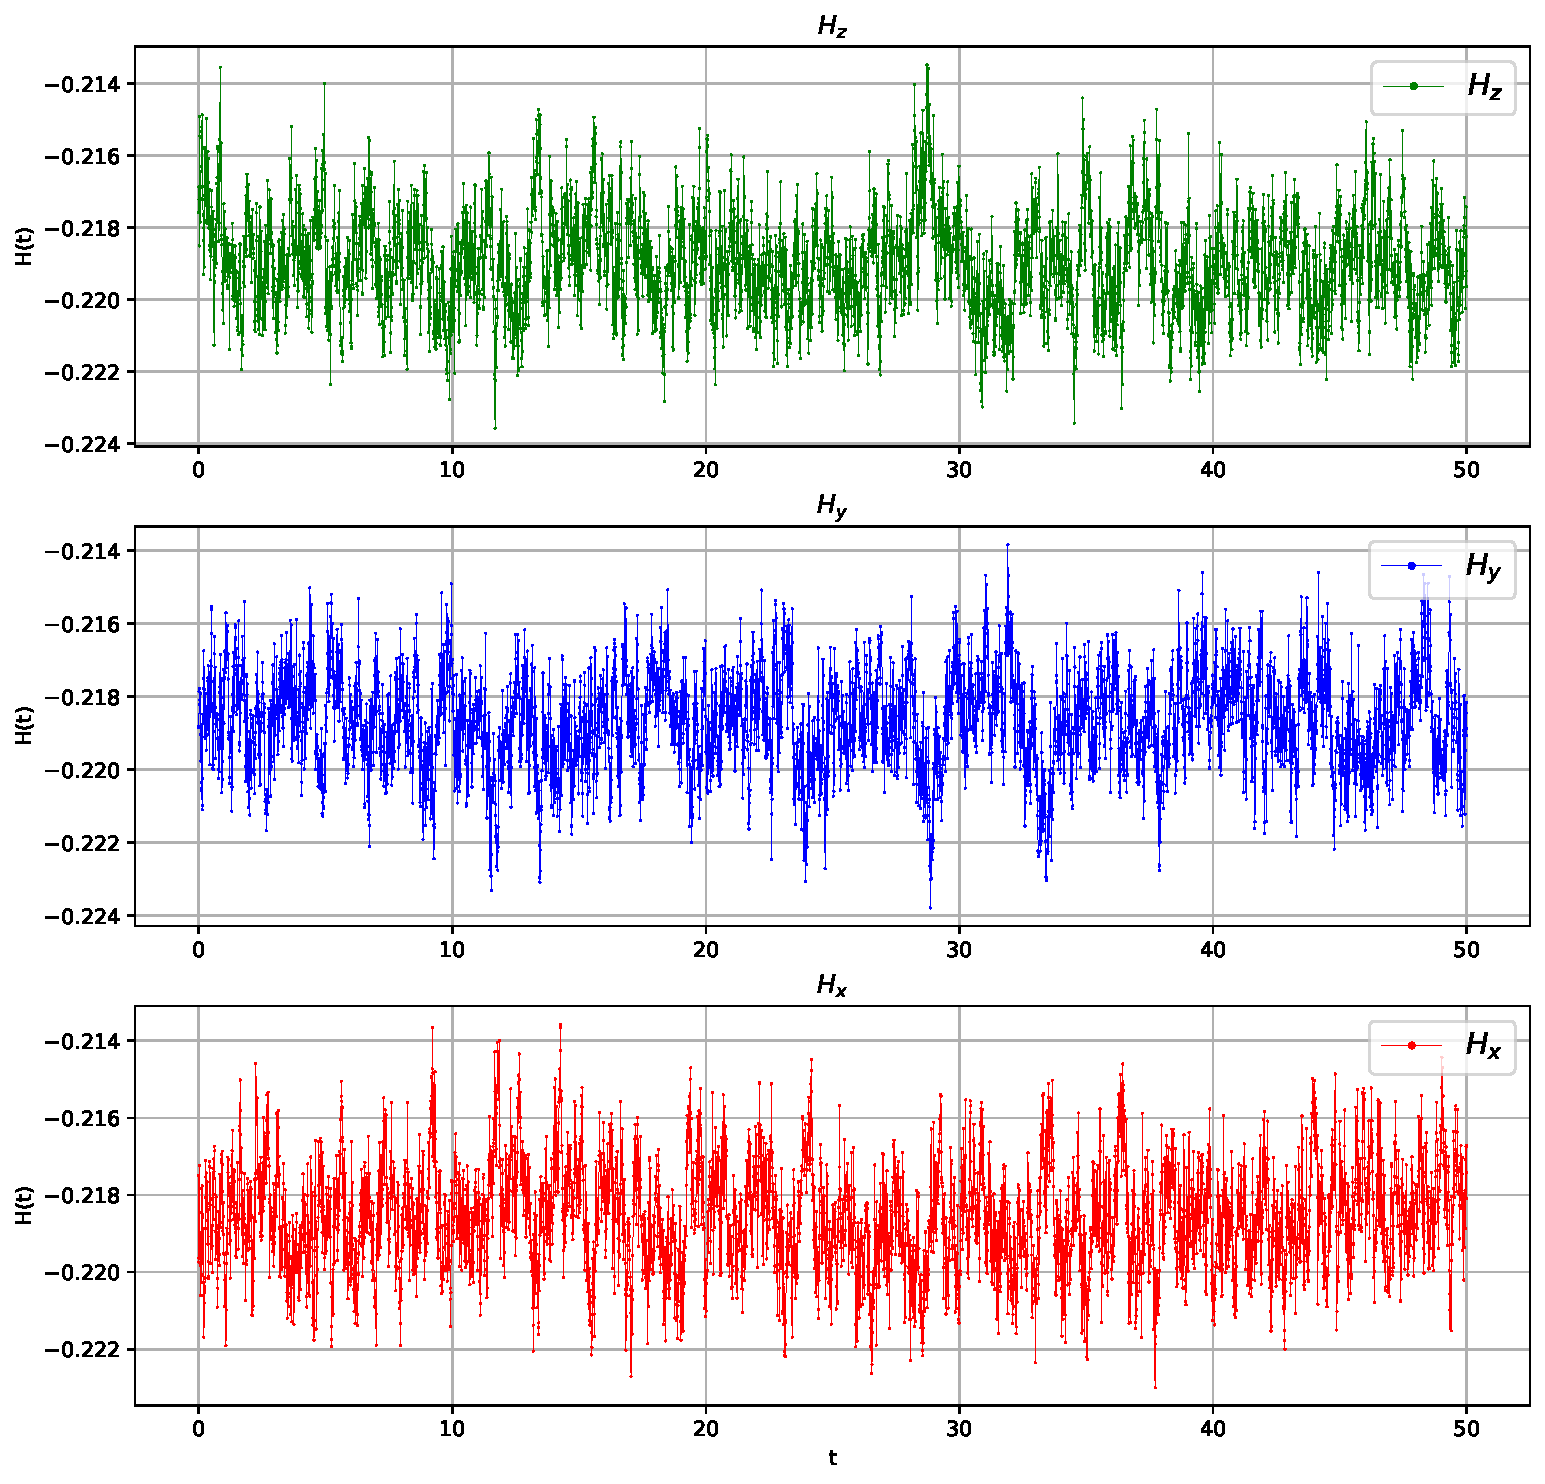
\includegraphics[width=0.9\textwidth]{../../Graficas/H_Boltzmann_xyz_1.pdf}
	\caption{valores de las funciones de Maxwell $H_x$, $H_y$ y $H_z$ con el tiempo.}
	\label{Fig:05}
\end{figure}

\begin{figure}[h!] \centering
	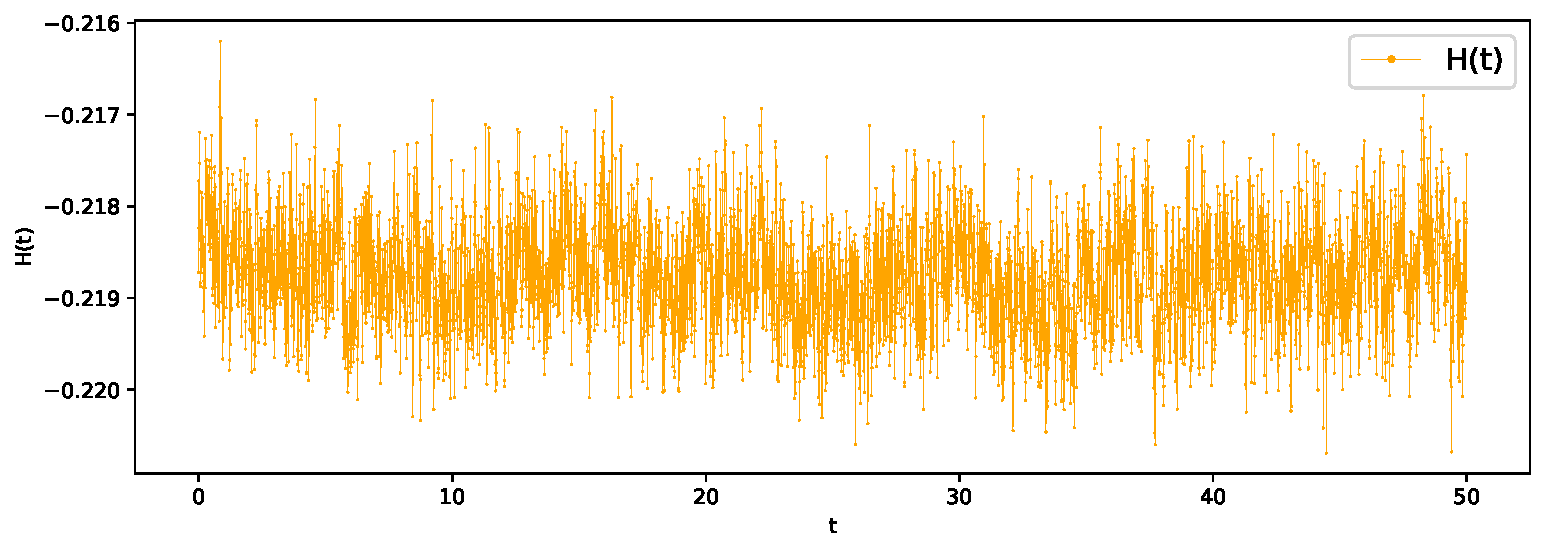
\includegraphics[width=0.9\textwidth]{../../Graficas/H_Boltzmann_1.pdf}
	\caption{Valor de la función de Maxwell $H(t)$ con el tiempo .}
	\label{Fig:06}
\end{figure}	
	
\newpage
	
\begin{figure}[h!] \centering
	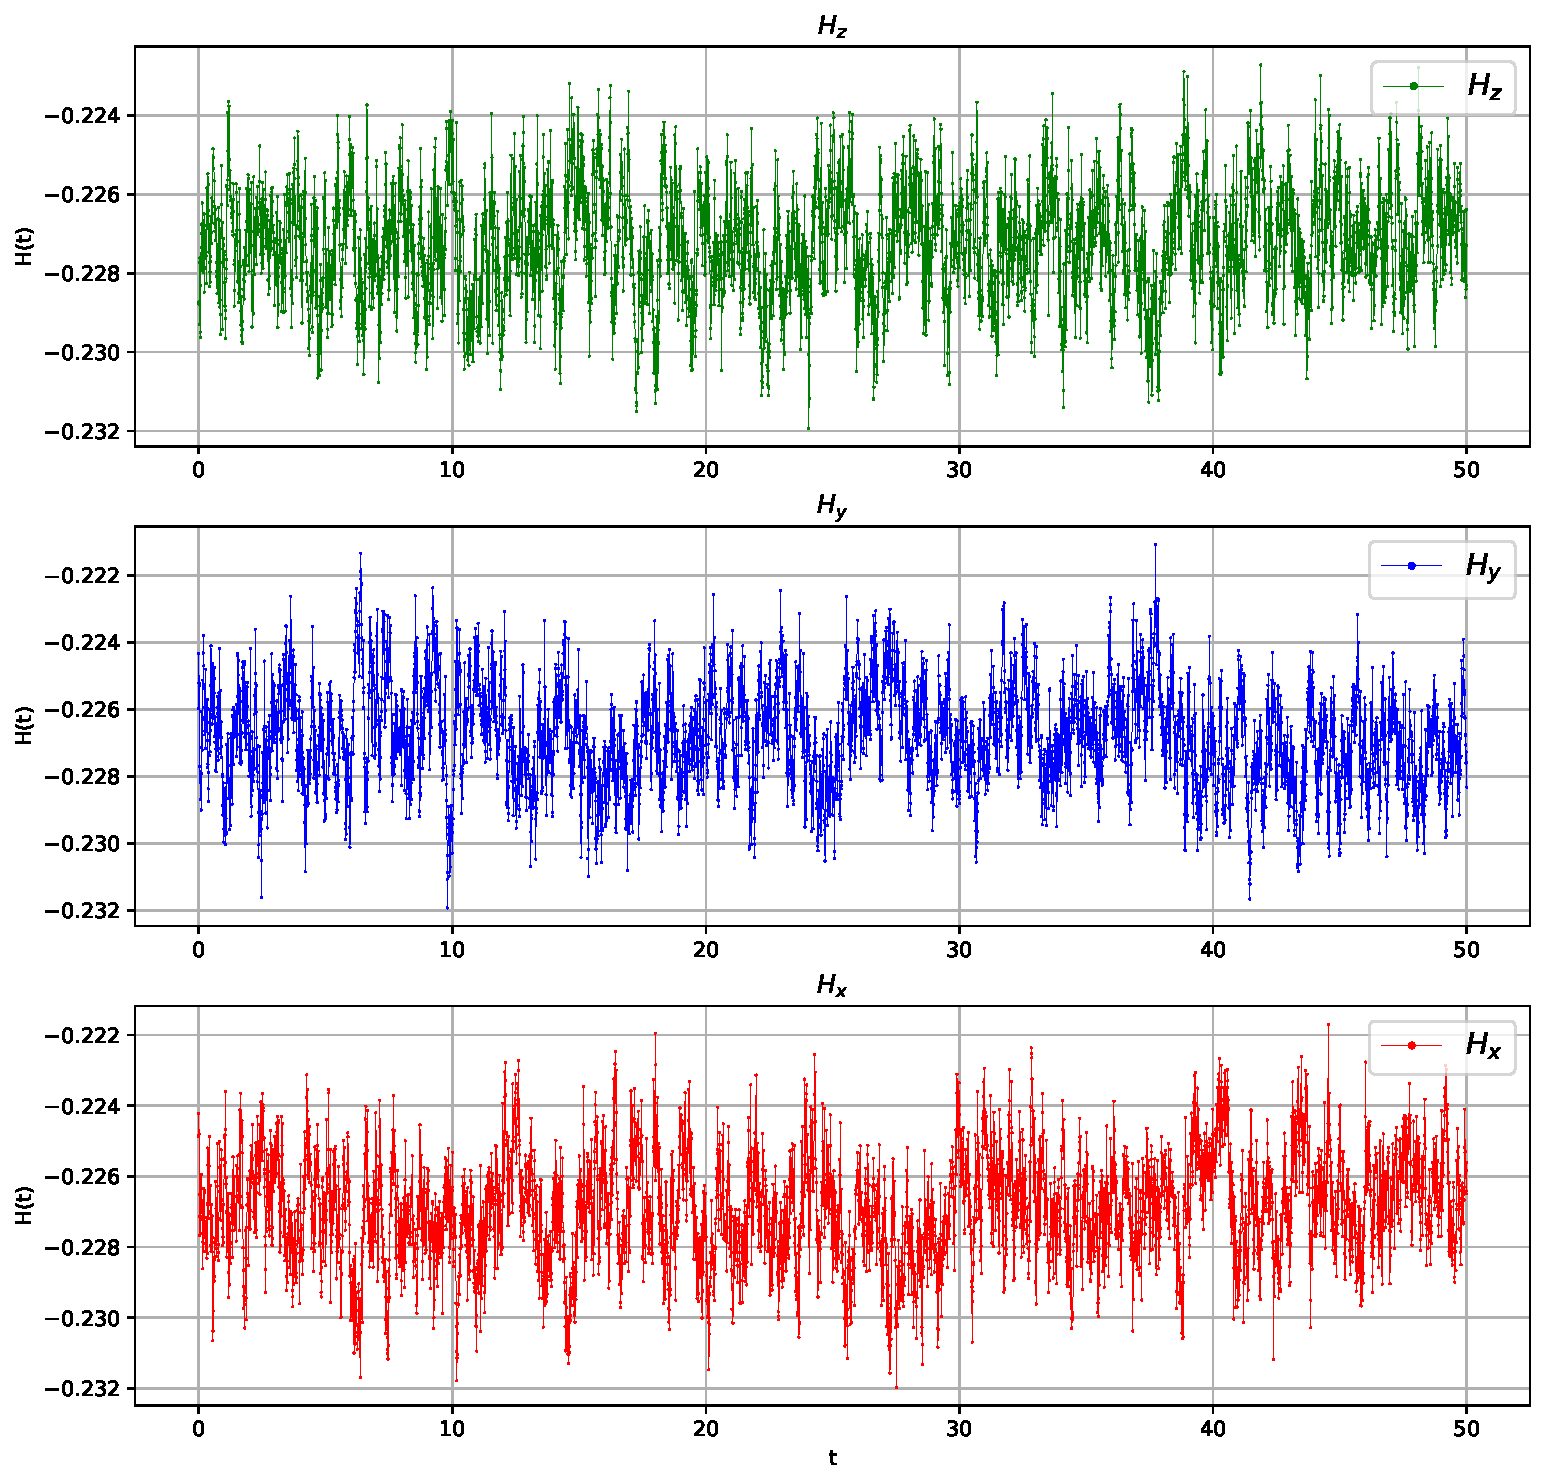
\includegraphics[width=0.9\textwidth]{../../Graficas/H_Boltzmann_xyz_2.pdf}
	\caption{valores de las funciones de Maxwell $H_x$, $H_y$ y $H_z$ con el tiempo.}
	\label{Fig:07}
\end{figure}
	
\begin{figure}[h!] \centering
	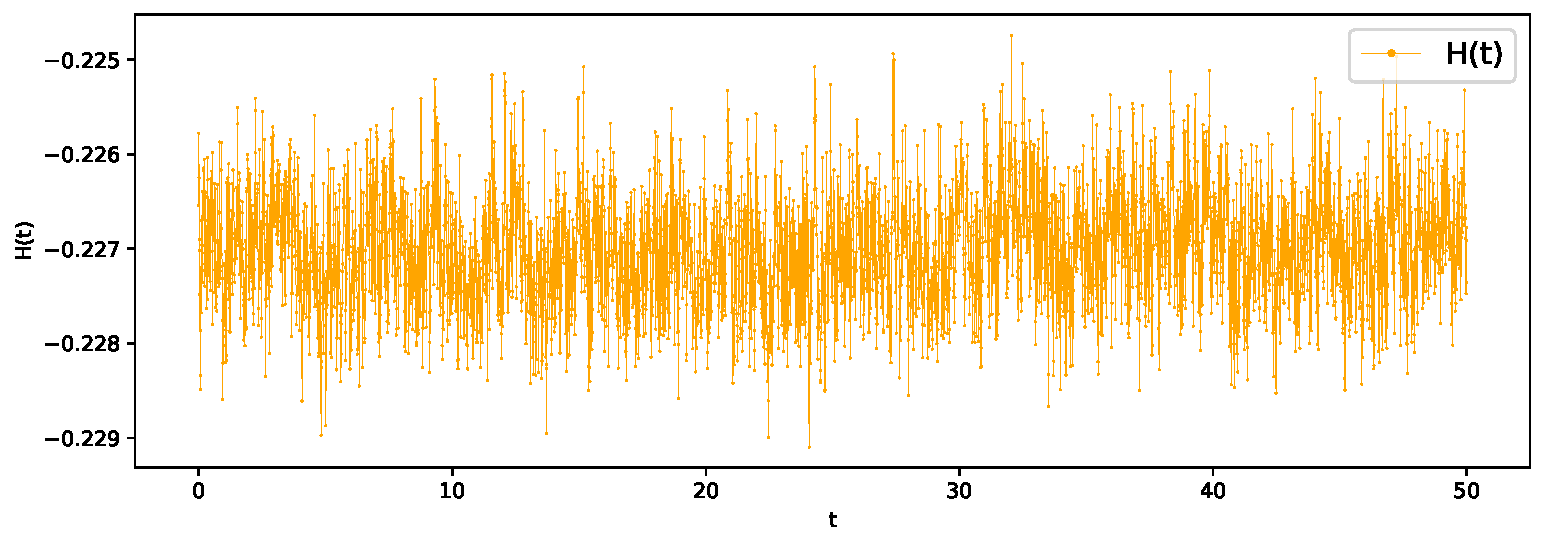
\includegraphics[width=0.9\textwidth]{../../Graficas/H_Boltzmann_2.pdf}
	\caption{Valor de la función de Maxwell $H(t)$ con el tiempo .}
	\label{Fig:08}
\end{figure}	
	
\newpage	

\section{Organización}

En este programa hemos usado 2 programas de fortran y 3 de python. Los programas de fortran son:

\begin{itemize}
	\item \textbf{Pro\_Funcion\_H}: lee los datos de las velocidades para cada interacción y genera un archivo con las H de Boltzmann para dichas velocidades. 
	\item \textbf{Pro\_Distribucion\_velocidades}: lee los datos de las velocidades para cada interacción y genera un archivo con los histogramas de cada una de las velocidades.
\end{itemize}
Los programas de python se usan únicamente para hacer las gráficas y dar los valores medios.
	
\section{Conclusiones}

Las conclusiones son sencillas: las dos simulaciones verifican las condiciones de equilibrio, lo cual es sorprendente, ya que la primera, aún viniendo de las posiciones de la equilibración de 5000 pasos, llega ya en equilibrio, verificando incluso una equilibración más estable. Cabe destacar que, a pesar de que si verifica la equilibración, no vamos a usarla para la posterior dinámica molecular, ya que la energía está bastante alejada de -575 (véase tabla \ref{Tab:01}).  \\

Es importante mencionar que el estudio de las condiciones de equilbiración es bastante escueto, ya que quizás lo ideal sería hacer más pasos y estudiar un conjunto de datos más extenso. También, debido a la cantidad de tiempo que requeriría su implementación, quedan sin hacer mejoras en la eficiencia de los algoritmos, así como el estudio de la distribución para $v$ módulo entre otras. 
	
	
\bibliography{Bibliografia.bib}
\bibliographystyle{unsrt}
	
	
\end{document}	
